\documentclass[14pt]{extbook}
\usepackage{multicol, enumerate, enumitem, hyperref, color, soul, setspace, parskip, fancyhdr} %General Packages
\usepackage{amssymb, amsthm, amsmath, bbm, latexsym, units, mathtools} %Math Packages
\everymath{\displaystyle} %All math in Display Style
% Packages with additional options
\usepackage[headsep=0.5cm,headheight=12pt, left=1 in,right= 1 in,top= 1 in,bottom= 1 in]{geometry}
\usepackage[usenames,dvipsnames]{xcolor}
\usepackage{dashrule}  % Package to use the command below to create lines between items
\newcommand{\litem}[1]{\item#1\hspace*{-1cm}\rule{\textwidth}{0.4pt}}
\pagestyle{fancy}
\lhead{Progress Quiz 4}
\chead{}
\rhead{Version A}
\lfoot{8448-1521}
\cfoot{}
\rfoot{Fall 2020}
\begin{document}

\begin{enumerate}
\litem{
Solve the radical equation below. Then, choose the interval(s) that the solution(s) belongs to.\[ \sqrt{8 x + 4} - \sqrt{3 x + 6} = 0 \]\begin{enumerate}[label=\Alph*.]
\item \( x \in [0.24,0.53] \)
\item \( x_1 \in [-3.33, -1.97] \text{ and } x_2 \in [-1.32,-0.08] \)
\item \( x \in [-3.33,-1.97] \)
\item \( \text{All solutions lead to invalid or complex values in the equation.} \)
\item \( x_1 \in [-0.84, 0.21] \text{ and } x_2 \in [-0.15,0.76] \)

\end{enumerate} }
\litem{
Solve the radical equation below. Then, choose the interval(s) that the solution(s) belongs to.\[ \sqrt{-8 x^2 - 35} - \sqrt{34 x} = 0 \]\begin{enumerate}[label=\Alph*.]
\item \( x \in [-2.3,-1.62] \)
\item \( \text{All solutions lead to invalid or complex values in the equation.} \)
\item \( x_1 \in [-2.76, -2.46] \text{ and } x_2 \in [-2.75,1.25] \)
\item \( x_1 \in [2.19, 3.63] \text{ and } x_2 \in [0.75,5.75] \)
\item \( x \in [-2.76,-2.46] \)

\end{enumerate} }
\litem{
Solve the radical equation below. Then, choose the interval(s) that the solution(s) belongs to.\[ \sqrt{72 x^2 + 4} - \sqrt{-34 x} = 0 \]\begin{enumerate}[label=\Alph*.]
\item \( x \in [-0.24,-0.21] \)
\item \( x \in [-0.26,-0.23] \)
\item \( x_1 \in [0.22, 0.23] \text{ and } x_2 \in [0.09,0.68] \)
\item \( x_1 \in [-0.26, -0.23] \text{ and } x_2 \in [-0.47,-0.18] \)
\item \( \text{All solutions lead to invalid or complex values in the equation.} \)

\end{enumerate} }
\litem{
Choose the equation of the function graphed below.
\begin{center}
    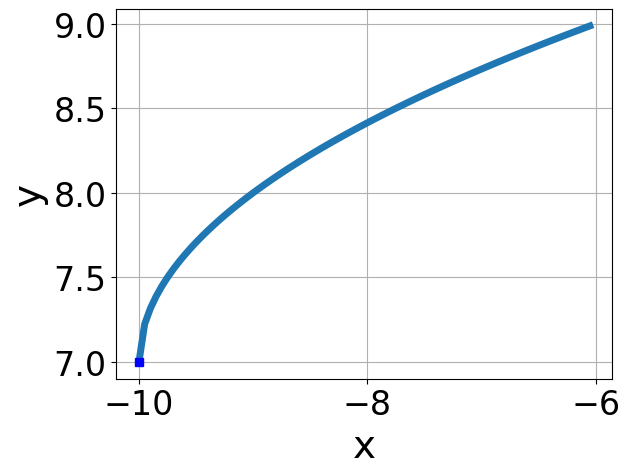
\includegraphics[width=0.5\textwidth]{../Figures/radicalGraphToEquationCopyA.png}
\end{center}
\begin{enumerate}[label=\Alph*.]
\item \( f(x) = \sqrt{x + 10} + 7 \)
\item \( f(x) = - \sqrt{x + 10} + 7 \)
\item \( f(x) = - \sqrt{x - 10} + 7 \)
\item \( f(x) = \sqrt{x - 10} + 7 \)
\item \( \text{None of the above} \)

\end{enumerate} }
\litem{
Choose the graph of the equation below.\[ f(x) = \sqrt[3]{x + 14} + 4 \]\begin{enumerate}[label=\Alph*.]
\begin{multicols}{2}\item 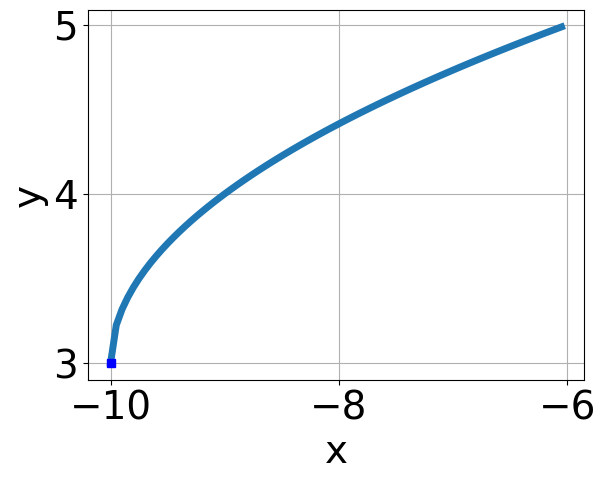
\includegraphics[width = 0.3\textwidth]{../Figures/radicalEquationToGraphAA.png}\item 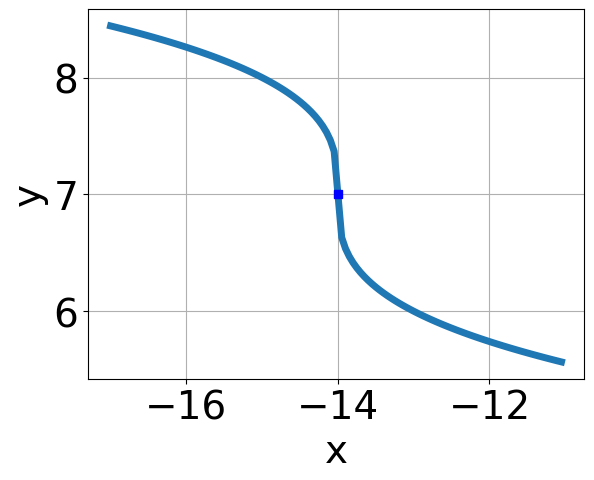
\includegraphics[width = 0.3\textwidth]{../Figures/radicalEquationToGraphBA.png}\item 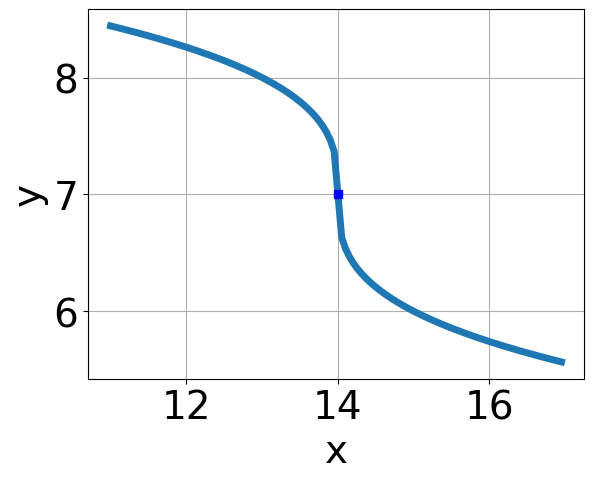
\includegraphics[width = 0.3\textwidth]{../Figures/radicalEquationToGraphCA.png}\item 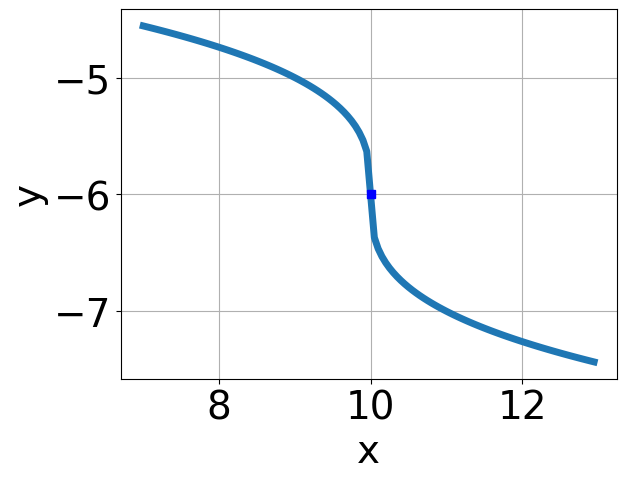
\includegraphics[width = 0.3\textwidth]{../Figures/radicalEquationToGraphDA.png}\end{multicols}\item None of the above.
\end{enumerate} }
\litem{
Choose the graph of the equation below.\[ f(x) = - \sqrt[3]{x + 6} + 3 \]\begin{enumerate}[label=\Alph*.]
\begin{multicols}{2}\item 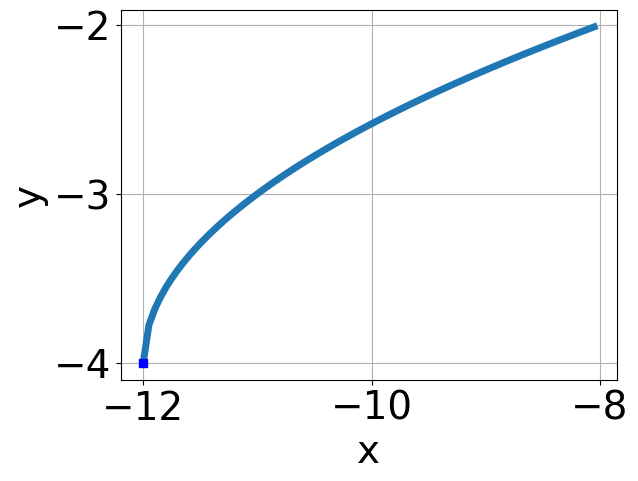
\includegraphics[width = 0.3\textwidth]{../Figures/radicalEquationToGraphCopyAA.png}\item 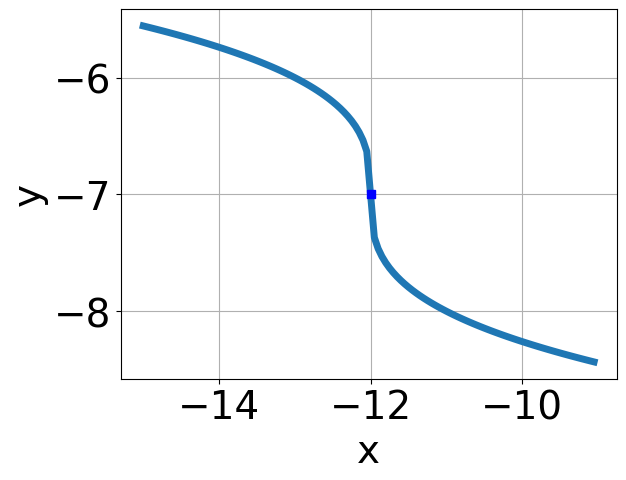
\includegraphics[width = 0.3\textwidth]{../Figures/radicalEquationToGraphCopyBA.png}\item 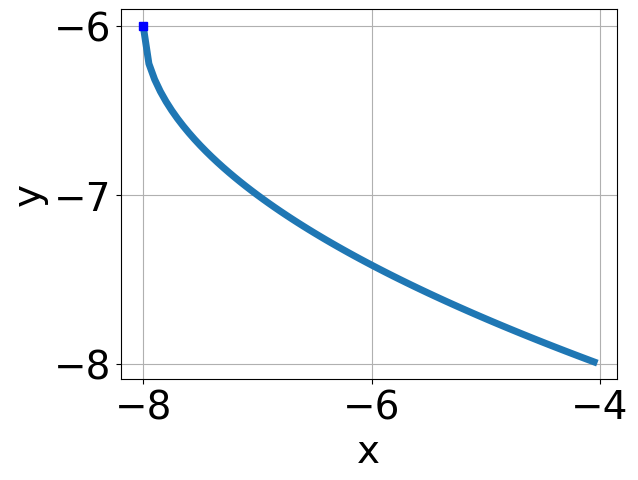
\includegraphics[width = 0.3\textwidth]{../Figures/radicalEquationToGraphCopyCA.png}\item 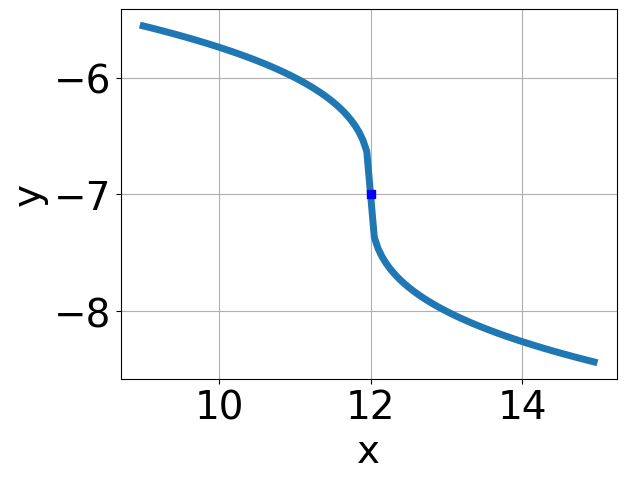
\includegraphics[width = 0.3\textwidth]{../Figures/radicalEquationToGraphCopyDA.png}\end{multicols}\item None of the above.
\end{enumerate} }
\litem{
What is the domain of the function below?\[ f(x) = \sqrt[4]{-8 x - 3} \]\begin{enumerate}[label=\Alph*.]
\item \( (-\infty, \infty) \)
\item \( [a, \infty), \text{where } a \in [-1.3, 1.8] \)
\item \( (-\infty, a], \text{ where } a \in [-1, 2.7] \)
\item \( [a, \infty), \text{where } a \in [-5, -1.9] \)
\item \( (-\infty, a], \text{where } a \in [-5.4, -1.7] \)

\end{enumerate} }
\litem{
What is the domain of the function below?\[ f(x) = \sqrt[6]{-5 x + 4} \]\begin{enumerate}[label=\Alph*.]
\item \( [a, \infty), \text{where } a \in [0.35, 0.85] \)
\item \( (-\infty, a], \text{where } a \in [0.96, 1.36] \)
\item \( (-\infty, \infty) \)
\item \( [a, \infty), \text{where } a \in [0.9, 1.36] \)
\item \( (-\infty, a], \text{ where } a \in [0.25, 0.93] \)

\end{enumerate} }
\litem{
Choose the equation of the function graphed below.
\begin{center}
    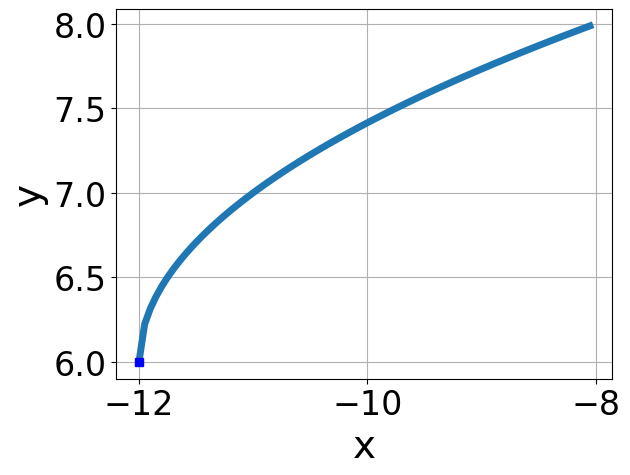
\includegraphics[width=0.5\textwidth]{../Figures/radicalGraphToEquationA.png}
\end{center}
\begin{enumerate}[label=\Alph*.]
\item \( f(x) = - \sqrt[3]{x + 8} - 7 \)
\item \( f(x) = \sqrt[3]{x + 8} - 7 \)
\item \( f(x) = - \sqrt[3]{x - 8} - 7 \)
\item \( f(x) = \sqrt[3]{x - 8} - 7 \)
\item \( \text{None of the above} \)

\end{enumerate} }
\litem{
Solve the radical equation below. Then, choose the interval(s) that the solution(s) belongs to.\[ \sqrt{-8 x - 5} - \sqrt{5 x - 4} = 0 \]\begin{enumerate}[label=\Alph*.]
\item \( x \in [-0.75,-0.63] \)
\item \( x_1 \in [-0.64, -0.57] \text{ and } x_2 \in [-0.8,0.5] \)
\item \( \text{All solutions lead to invalid or complex values in the equation.} \)
\item \( x \in [-0.15,-0.06] \)
\item \( x_1 \in [-0.64, -0.57] \text{ and } x_2 \in [0.4,3.2] \)

\end{enumerate} }
\end{enumerate}

\end{document}